\let\clearpage\relax
\begin{textbox}{\href{https://compneuro.neuromatch.io/tutorials/W1D3_GeneralizedLinearModels/student/W1D3_Tutorial1.html}{Generalized Linear Models } }
\begin{subbox}{subbox}{Create design matrix}
\scriptsize

To create the \textbf{design matrix} which organizes the stimulus intensities in matrix form such that the $i$th row has the stimulus frames preceding timepoint $i$.

In this example, we will create the design matrix $\mathbf{X}$ using $d=25$ time lags. That is, $\mathbf{X}$ should be a $T \times d$ matrix. $d = 25$  is a choice we're making based on our prior knowledge of the temporal window that influences RGC responses. 
Here, spike count is $\mathbf{Y}$ is predicted from out stimulus $\mathbf{X}$,
\centering
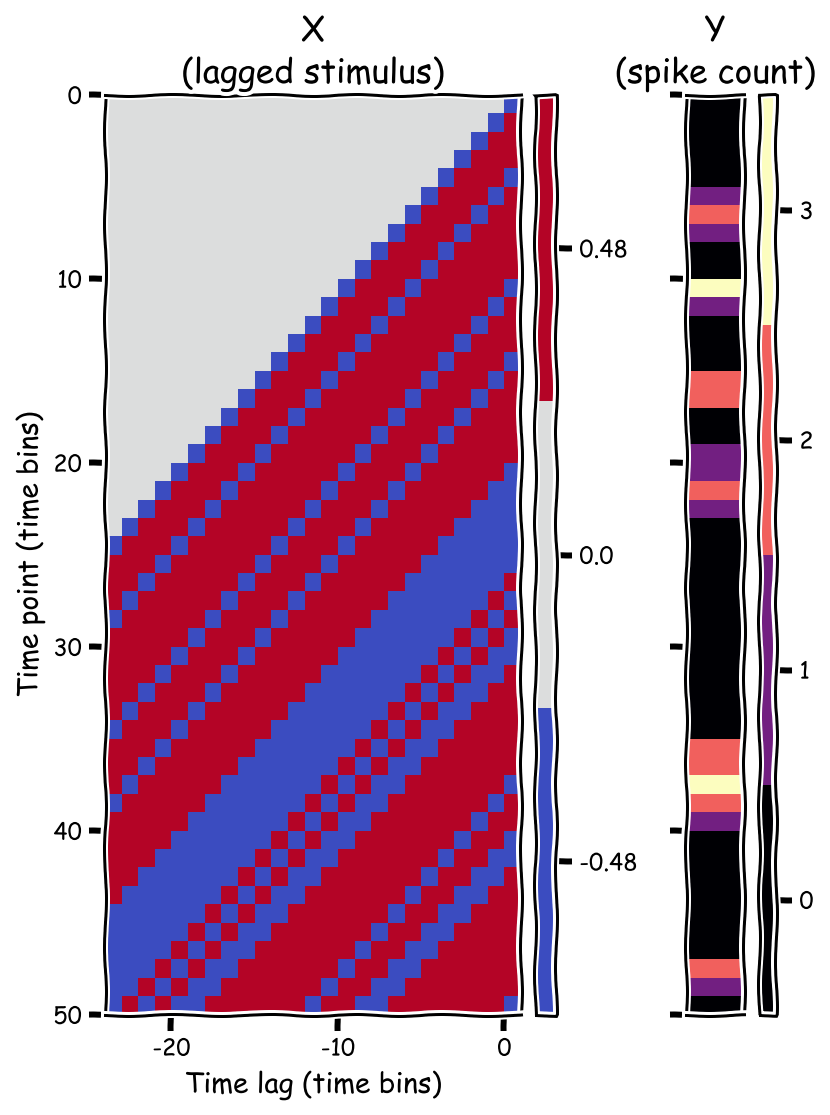
\includegraphics[scale=0.11]{Figures/GLM/GLMFigure1.png}
\end{subbox}

\begin{subbox}{subbox}{Fit Linear-Gaussian regression model 
}
\scriptsize{The maximum likelihood estimate of $\theta$ in this model can be solved analytically using the equation:

\begin{align}
\boldsymbol{\hat \theta} = (\mathbf{X}^{\top}\mathbf{X})^{-1}\mathbf{X}^{\top}\mathbf{y}.
\end{align}}
The resulting maximum likelihood filter estimates are:
\centering
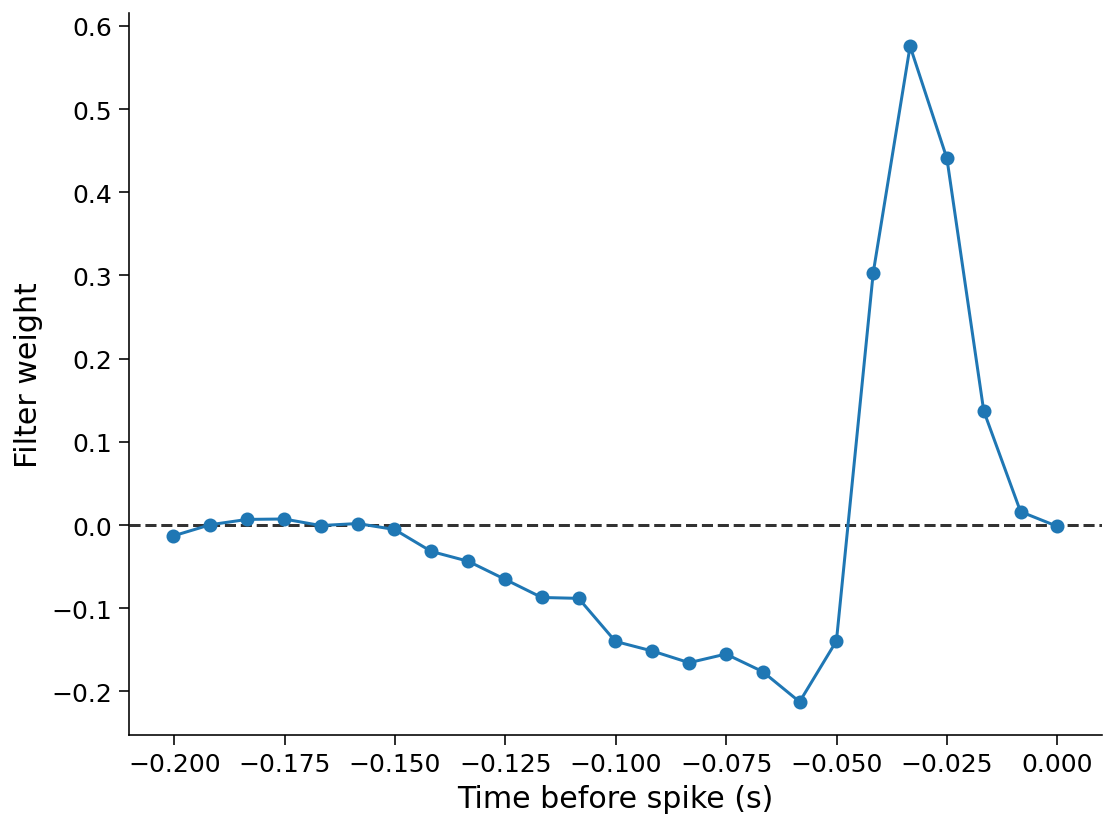
\includegraphics[scale=0.2]{Figures/GLM/GLMFigure2.png}
\end{subbox}
\end{textbox}
%%%%%%%%%%%%%%%%%%%%%%%%%%%%%%%%%%%%%%%%%%%%%%%%%%
%%%%%%%%%%%%%%%%%%%%%%%%%%%%%%%%%%%%%%%%%%%%%%%%%%
\begin{textbox}{\href{https://compneuro.neuromatch.io/tutorials/W1D3_GeneralizedLinearModels/student/W1D3_Tutorial1.html}{Generalized Linear Models } }
\begin{subbox}{subbox}{Poisson regression}
\scriptsize
Poisson regression is a generalized linear model form of regression analysis used to model count data, like spikes.
In the Poisson GLM,
\begin{align}
\log P(\mathbf{y} \mid \mathbf{X}, \theta) = \sum_t \log P(y_t \mid \mathbf{x_t},\theta),
\end{align}
where
\begin{align}
P(y_t \mid \mathbf{x_t}, \theta) = \frac{\lambda_t^{y_t}\exp(-\lambda_t)}{y_t!} \text{, with rate } \lambda_t = \exp(\mathbf{x_t}^{\top} \theta).
\end{align}

Now, taking the log likelihood for all the data we obtain:
$\log P(\mathbf{y} \mid X, \theta) = \sum_t( y_t \log\left(\lambda_t) - \lambda_t - \log(y_t !)\right).$

Because we are going to minimize the negative log likelihood with respect to the parameters $\theta$, we can ignore the last term that does not depend on $\theta$. For faster implementation, let us rewrite this in matrix notation:

\begin{align}
\mathbf{y}^{\top} \log(\mathbf{\lambda}) - \mathbf{1}^{\top} \mathbf{\lambda} \text{, with  rate } \mathbf{\lambda} = \exp(\mathbf{X} \theta)
\end{align}

Finally, don't forget to add the minus sign for your function to return the negative log likelihood.

\centering
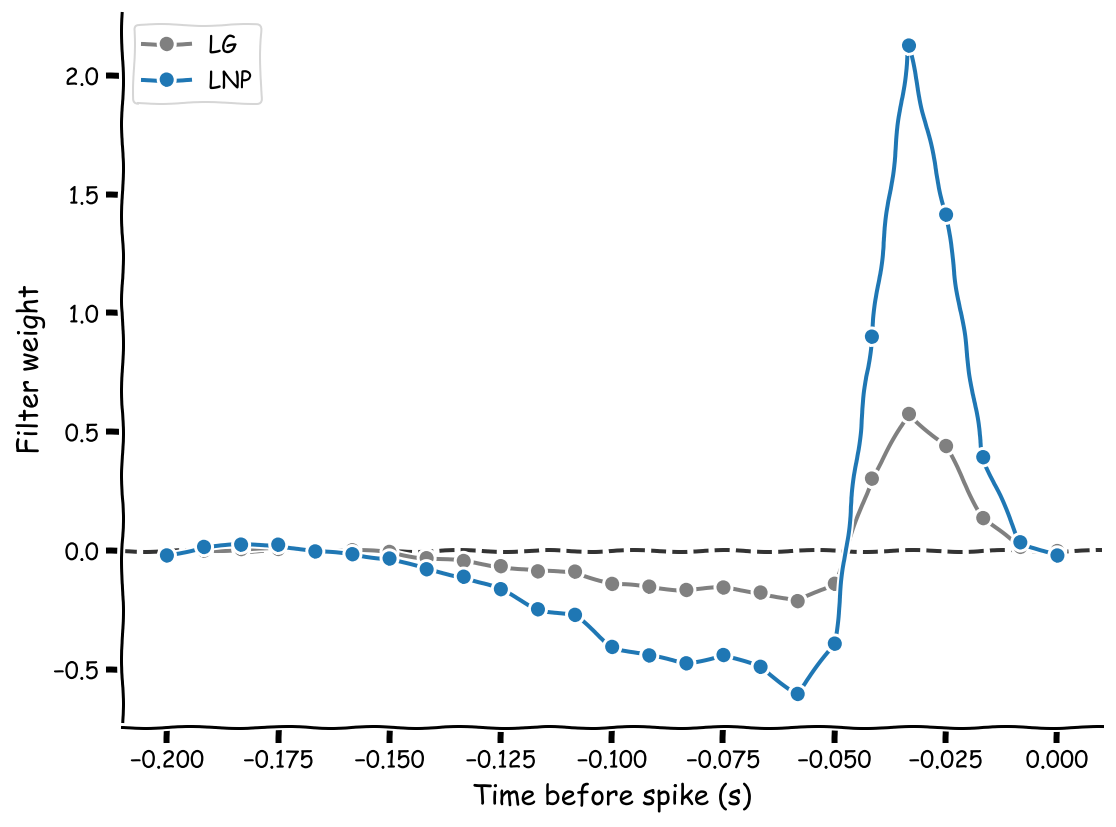
\includegraphics[scale=0.1]{Figures/GLM/GLMFigure3.png}
\end{subbox}

\begin{subbox}{subbox}{Spike Prediction 
}

\centering
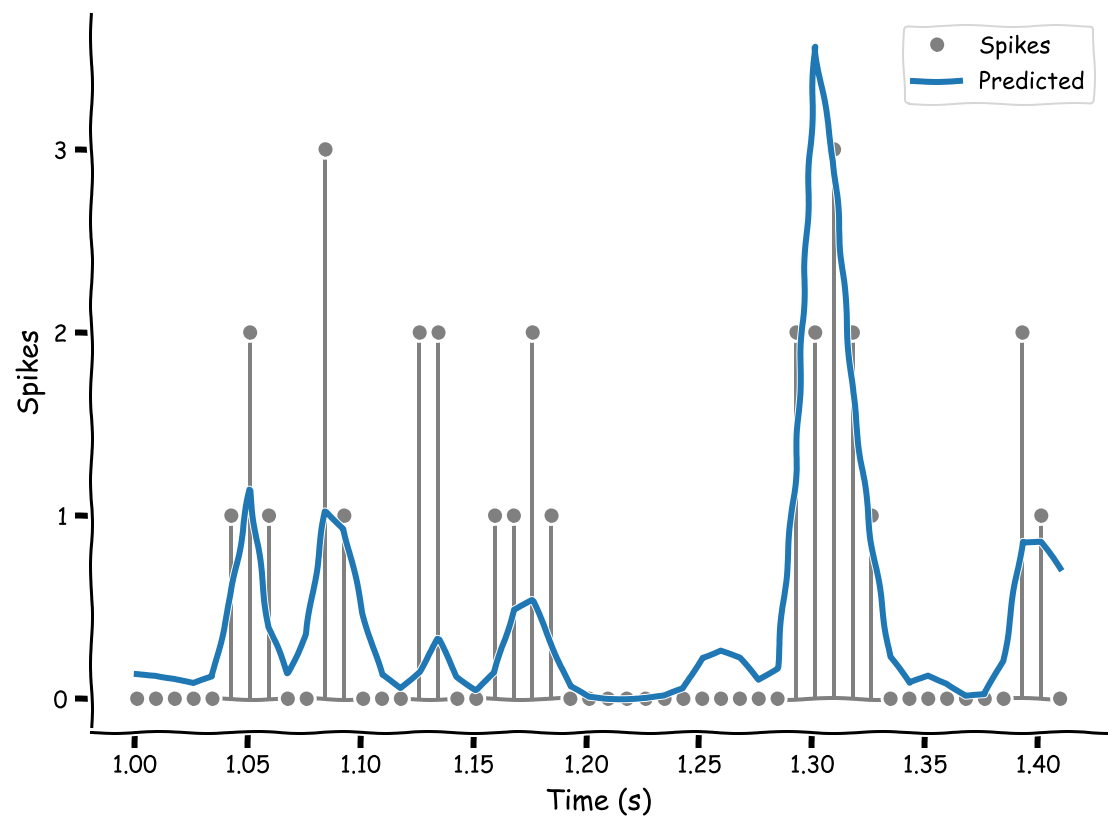
\includegraphics[scale=0.1]{Figures/GLM/GLMFigure4.png}
\end{subbox}
\end{textbox}
%%%%%%%%%%%%%%%%%%%%%%%%%%%%%%%%%%%%%%%%%%%%%%%%%%
%%%%%%%%%%%%%%%%%%%%%%%%%%%%%%%%%%%%%%%%%%%%%%%%%%
\begin{textbox}{\href{https://compneuro.neuromatch.io/tutorials/W1D3_GeneralizedLinearModels/student/W1D3_Tutorial2.html}{Generalized Linear Models } }
\begin{subbox}{subbox}{Logistic regression}
\scriptsize
Logistic Regression is a binary classification model. It is a GLM with a logistic link function and a Bernoulli (i.e. coinflip) noise model.
The fundamental input/output equation of logistic regression is:

\begin{align}
\hat{y} \equiv p(y=1|x,\theta) = \sigma(\theta^Tx)
\end{align}

Note that we interpret the output of logistic regression, $\hat{y}$, as the probability that $y = 1$ given inputs $x$ and parameters $\theta$.

Here $\sigma()$ is a "squashing" function called the sigmoid function or logistic function. Its output is in the range $0 \leq y \leq 1$. It looks like this:

\begin{align}
\sigma(z) = \frac{1}{1 + \textrm{exp}(-z)}
\end{align}
Recall that $z = \theta^T x$. The parameters decide whether $\theta^T x$ will be very negative, in which case $\sigma(\theta^T x)\approx 0$, or very positive, meaning  $\sigma(\theta^T x)\approx 1$.

\centering
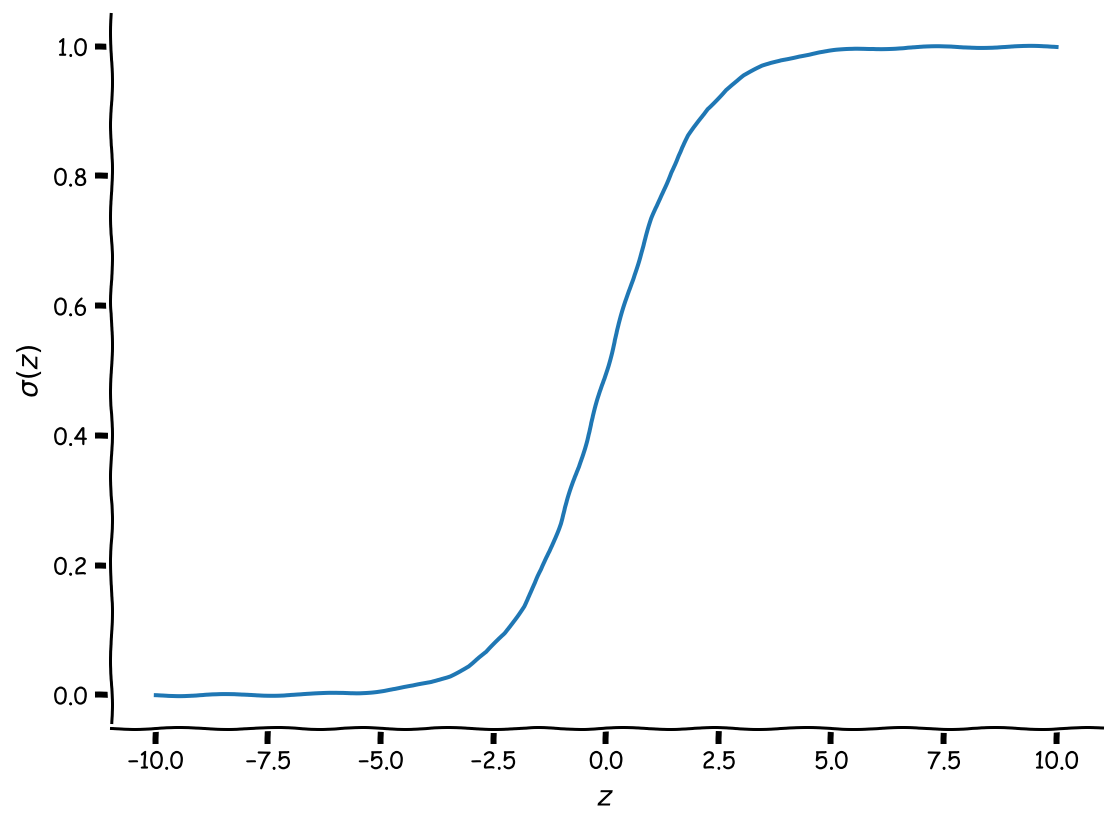
\includegraphics[scale=0.07]{Figures/GLM/GLMFigure5.png}
\end{subbox}

\begin{subbox}{subbox}{Regularisation 
}
\scriptsize
Regularization forces a model to learn a set solutions you a priori believe to be more correct, which reduces over-fitting because it doesn't have as much flexibility to fit idiosyncrasies in the training data. This adds model bias, but it's a good bias because you know (maybe) that parameters should be small or mostly 0.

\textbf{$L_2$ regularization}\\
Regularization comes in different flavors. A very common one uses an $L_2$ or "ridge" penalty. This changes the objective function to
\begin{align}
-\log\mathcal{L}'(\theta | X, y)=
-\log\mathcal{L}(\theta | X, y) +\frac\beta2\sum_i\theta_i^2,
\end{align}
where $\beta$ is a \textit{hyperparameter} that sets the \textit{strength} of the regularization.

\end{subbox}

\end{textbox}
%%%%%%%%%%%%%%%%%%%%%%%%%%%%%%%%%%%%%%%%%%%%%%%%%%
%%%%%%%%%%%%%%%%%%%%%%%%%%%%%%%%%%%%%%%%%%%%%%%%%%
\begin{textbox}{\href{https://compneuro.neuromatch.io/tutorials/W1D3_GeneralizedLinearModels/student/W1D3_Tutorial2.html}{Generalized Linear Models } }
\begin{subbox}{subbox}{Logistic regression}
\scriptsize
Logistic Regression is a binary classification model. It is a GLM with a logistic link function and a Bernoulli (i.e. coinflip) noise model.
The fundamental input/output equation of logistic regression is:

\begin{align}
\hat{y} \equiv p(y=1|x,\theta) = \sigma(\theta^Tx)
\end{align}

Note that we interpret the output of logistic regression, $\hat{y}$, as the probability that $y = 1$ given inputs $x$ and parameters $\theta$.

Here $\sigma()$ is a "squashing" function called the sigmoid function or logistic function. Its output is in the range $0 \leq y \leq 1$. It looks like this:

\begin{align}
\sigma(z) = \frac{1}{1 + \textrm{exp}(-z)}
\end{align}
Recall that $z = \theta^T x$. The parameters decide whether $\theta^T x$ will be very negative, in which case $\sigma(\theta^T x)\approx 0$, or very positive, meaning  $\sigma(\theta^T x)\approx 1$.

\centering
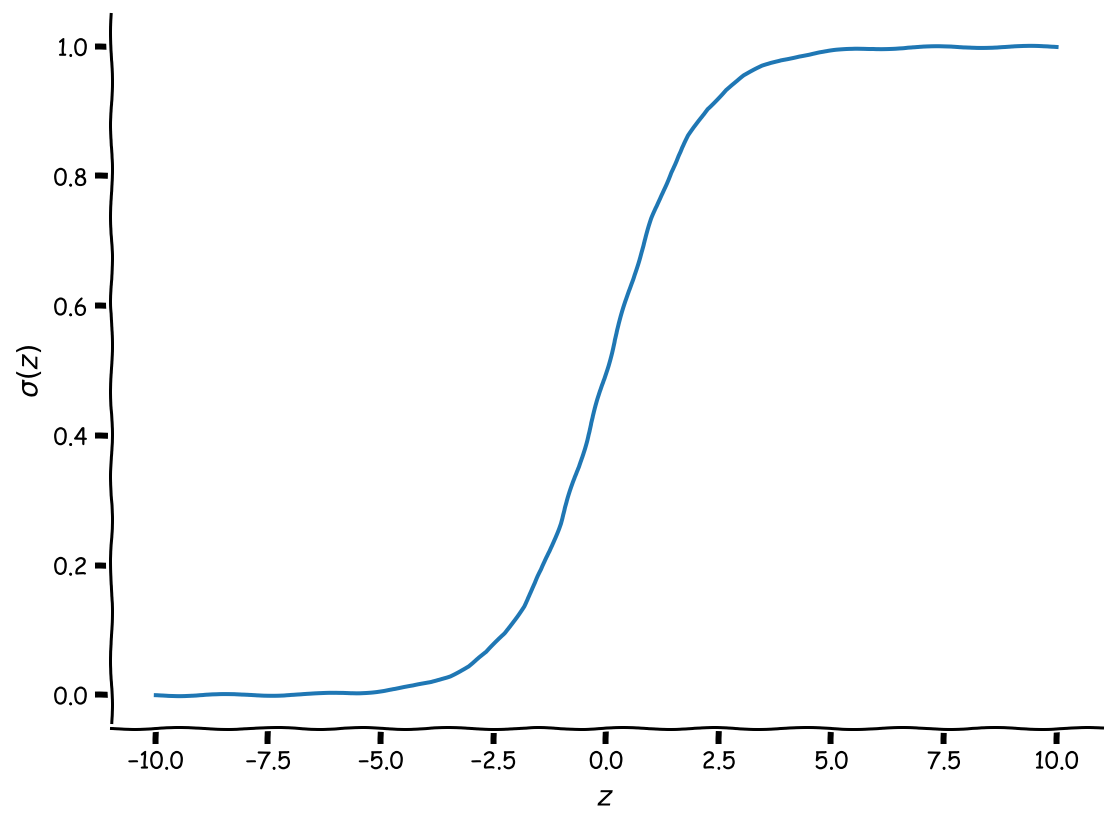
\includegraphics[scale=0.07]{Figures/GLM/GLMFigure5.png}
\end{subbox}

\begin{subbox}{subbox}{Regularisation 
}
\scriptsize
Regularization forces a model to learn a set solutions you a priori believe to be more correct, which reduces over-fitting because it doesn't have as much flexibility to fit idiosyncrasies in the training data. This adds model bias, but it's a good bias because you know (maybe) that parameters should be small or mostly 0.

\textbf{$L_2$ regularization}\\
Regularization comes in different flavors. A very common one uses an $L_2$ or "ridge" penalty. This changes the objective function to
\begin{align}
-\log\mathcal{L}'(\theta | X, y)=
-\log\mathcal{L}(\theta | X, y) +\frac\beta2\sum_i\theta_i^2,
\end{align}
where $\beta$ is a \textit{hyperparameter} that sets the \textit{strength} of the regularization.

\end{subbox}

\end{textbox}